\documentclass[letterpaper]{article}
\usepackage{alltt}
\usepackage{graphicx}
\usepackage{xspace}
\usepackage{color}
\definecolor{linkcolor}{RGB}{16,65,69}

\newcommand{\ttt}[1]{\texttt{#1}}
\newcommand{\projname}{\ttt{bt}\xspace}

\newenvironment{monospace}{\begin{quote}\begin{alltt}}{\end{alltt}\end{quote}}

\author{Joe Colosimo \\ \small{colosimo@mit.edu} \\ Group 6}
\date{\today}

\usepackage[colorlinks=true, linkcolor=linkcolor]{hyperref}
\usepackage{rotating}
\title{\projname{} - A Realtime Beat Tracker \\ Final Report}
\begin{document}

\maketitle

\section{Primary Objective}
    \projname is a live beat tracker --- a device that reads a stream of music
    and, in realtime, makes a guess at its tempo.  

    Beat analysis is an important field of audio signal processing.  It's used
    in a variety of applications in the music universe.  For example, DJ
    software finds the tempo and beat locations of the tracks in the user's
    library beforehand in order to make synchronizing two playing tracks a
    straightforward process.  It's also used in audio-controlled lighting to
    generate complex displays that react to music.

    Most of the time, beat analysis is done before its information is actually
    needed.  As a result, these preprocessing algorithms (there are numerous)
    can be very accurate.


\section{Background}

    Realtime tempo estimation of a live stream is a difficult problem to solve,
    especially compared to a pre-processing-based approach.  In this case,
    we're looking not only to accurately identify a best estimate for the
    tempo, but also to converge on that estimate as quickly as possible.

    One algorithm involves trying to classify portions of a music stream as
    ``beats" and then tries to match those beats against one of many possible
    tempos, eventually narrowing in on a most likely candidate.  This includes
    creating a series of phase-locking metronomes, each running at a different
    tempo, and trying to match detected beats to subdivision of each metronome.
    It's as though we have purchased a hundred or so physical metronomes, put
    someone in front of each metronome, played a stream of music, and had each
    person reset their metronome when they heard a beat --- the difference is
    that we are able to measure just how far each metronomes was off from that
    beat and keep a running average of that value.



\section{Why Dedicated Hardware?}

    This algorithm is more of an entertaining novelty than anything else;
    nobody would actually use it in a real product.  But it does offer some
    interesting ideas with respect to parallelism.  Namely, dedicated hardware
    offers the ability to instantiate, for example, 60 or 70 different
    metronomes with very precise timing, all running independently of one
    another.  This would not be possible using conventional CPU architecture --
    most threaded models lose precision after just a few metronomes.
    Furthermore, realtime beat classification is a challenging algorithm to
    implement on most CPUs, even though there are often plenty of clock cycles
    between audio samples.  Although this project does not use a
    frequency-aware beat classification algorithm, it one were to switch to it,
    one would surely desire dedicated hardware for taking large FFTs.


\section{High Level Design}
    
    Figure~\ref{fig:architecture} illustrates the overall
    architecture of the system.

    \begin{figure}
        \centering
        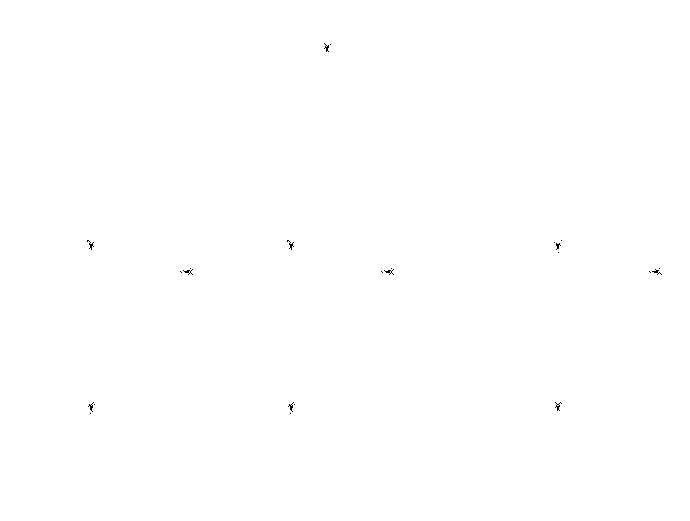
\includegraphics{fig/architecture.pdf}
        \caption{\projname algorithm architecture}
        \label{fig:architecture}
    \end{figure}

    The system starts off by instantiating metronomes with a wide range of
    tempos.  The number of metronomes is limited by the resource constraints of
    the system.  They all wait for the beat classifier to seed them with an
    initial guess at a beat, at which point they start running.  After this
    initialization phase, the metronomes keep time, each at their own tempo,
    and when the beat classifier detects a beat in the audio, it delivers a
    message to all of the metronomes stating the likelihood that the event it
    just saw was a beat.  The metronomes then all adjust their phase linearly
    with the probability that the beat classifier thought it was correct and
    report their current phase difference to the metronome bank controller.

    In this manner, metronomes whose tempo is different from the stream's real
    tempo will consistently report large phase errors, while those closer to
    the real tempo will report smaller phase errors.  We can then use these
    results to generate a probability distribution for the actual tempo.
    Optionally, after a period of convergence, we can ``zoom in" on the
    possible tempos, trying smaller and smaller increments around the most
    likely tempo until we converge on a reasonable result.  This project does
    not include that features because enough metronomes were instantiated to
    fit a large range of tempos with per-BPM precision.


\section{Testing}

    A Spartan 3A-N evaluation board was chosen as it was easily available.
    While this FPGA is realitvely weak, it was able to perform most of the
    intended design without issue.  It has an onboard ADC, so a small
    DC-biasing circuit with an audio jack was designed and attached to the
    board, as shown in Figures~\ref{fig:dcbias} and \ref{fig:dcbiasbrd}.  The
    overall setup is shown in Figure~\ref{fig:setup}.

    \begin{figure}
        \centering
        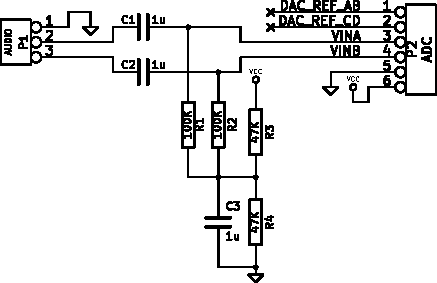
\includegraphics{fig/dcbias.pdf}
        \caption{DC biasing circuit schematic}
        \label{fig:dcbias}
    \end{figure}

    \begin{figure}
        \centering
        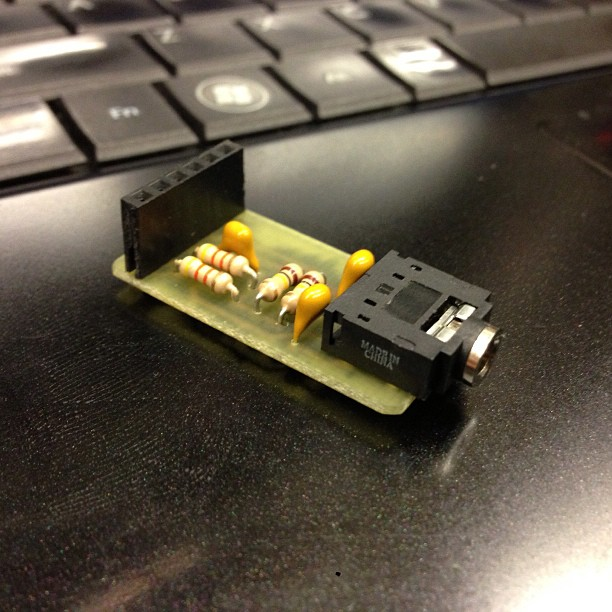
\includegraphics[scale=0.25]{fig/dcbiasbrd.jpg}
        \caption{DC biasing circuit board}
        \label{fig:dcbiasbrd}
    \end{figure}

    \begin{figure}
        \centering
        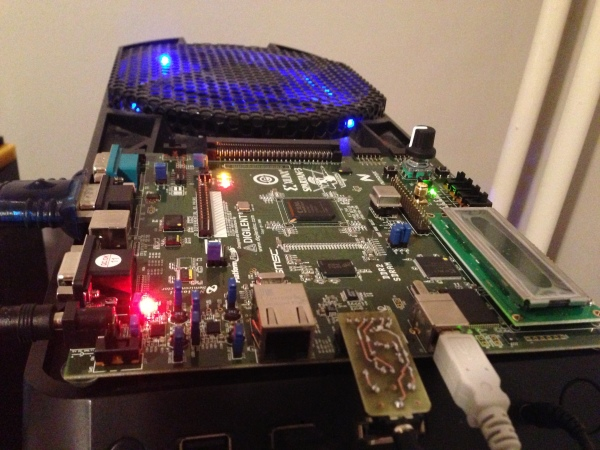
\includegraphics[scale=0.5]{fig/setup.jpg}
        \caption{FPGA setup}
        \label{fig:setup}
    \end{figure}

    Live audio was fed into the FPGA and the serial stream was read back into
    the computer.

    The simulation testbench operated in much the same way.  Samples were read
    from a data file and fed in with the appropriate clock subdivision.  Output
    samples were then recorded to a new file that could be parsed with a Python
    script.


\section{Microarchitecture}
    \subsection{Top Level}

        The top level module of \projname{} handles inter-module communication as
        well as sample injection and hardware output.

        \subsubsection{Interface to Hardware Architecture}

        The hardware produces audio samples and then requires a handshake to read
        the sample.  The underlying hardware architecture is shown in
        Figure~\ref{fig:hwarch}.  From the hardware side, the
        \ttt{sample\_injector} module
        provides the following signals:

        \begin{center}
        \begin{tabular}{|r|l|}
            \hline
            \ttt{sample} & \ttt{out std\_logic\_vector(13 downto 0)} \\ \hline
            \ttt{sample\_rdy} & \ttt{out std\_logic} \\ \hline
            \ttt{sample\_rd} & \ttt{in std\_logic} \\ \hline
        \end{tabular}
        \end{center}

        \begin{figure}
            \centering
            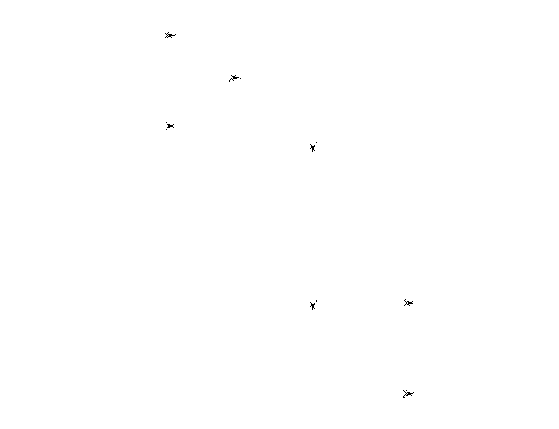
\includegraphics{fig/hwarch.pdf}
            \caption{hardware architecture}
            \label{fig:hwarch}
        \end{figure}

        \projname{} therefore waits for input \ttt{sample\_rdy} to go high, at
        which point it captures \ttt{sample} and asserts \ttt{sample\_rd = '1'} for
        one clock cycle.  It enqueues the sample to the beat classifier's input
        FIFO through its put method.

        The output of the top module is a FIFO that talks to the underlying
        hardware.  With each detected beat, the FIFO is filled with the phase
        offsets of all of the metronomes and flushed via the serial controller.


    \subsection{Beat Classifier}

        The beat classifier handles the process of receiving injected audio samples
        and determining when the audio stream has likely produced a beat.  It
        operates as a server.  On the put side, we inject samples.  On the get
        side, we receive beat events.


        \subsubsection{Operation}
            
        The beat classification algorithm essentially compares the local energy of
        a small sample window to the average energy of a much larger window.  If
        there is significant deviation of the local energy from the average energy
        (either positive or negative), then the beat classifier reports that it saw
        a beat.

        It runs a round of this every time it receives a sample via its
        \ttt{InjectSample} method, described below.  When a new sample has been
        presented, it computes this instantaneous energy of the sample, by squaring
        it and accumulates this to the \ttt{cur\_energy} register.  When $N_L$ of
        such samples are accumulated, we are ready to compare the local energy with
        the average energy, which is held in the \ttt{avg\_energy} register.  If
        the local energy is different from the average energy by a factor $F$, we
        report a beat by setting a register valid as described in
        Section~\ref{sec:bc:metif}.

        We also keep a list of the last $N_E$ energy values so that we can
        perform an arithmetic mean to calculate the average energy.  With each
        new energy, we ``kick out" the oldest value out of the average (by
        subtracting it) and add in the newest value.

        
        \subsubsection{Tunable Parameters}

        There are a few parameters here that can be fine-tuned.

        $N_L$ basically asks "how many samples corresponds to local energy?".  If
        it's too small, we may not get a good enough estimate of the signal energy
        at any given point, but if it's too large, then we could be including a
        beat with non-beat portion of the spectrum.  Experiments suggest that $N_L
        \approx 1000$ works well.

        $F$ determines just how different the local energy has to be from the
        average energy for a beat to be considered.  In practice, if we were to
        think of the ratio of local energy to average energy, $F$ usually works
        well at about 1.2 or 1.3.  However, this can vary by genre.  This is why I
        would eventually like to be able to compute the variance of local energies
        to determine a best fit for F.

        $N_E$ determines how many energy components make up the average energy.
        We target around 1 second's worth of samples because biologically, the
        human ear has been found to compare sound energy to a history of about
        1 second.


        \subsubsection{Put Interface}

        The module has a very small FIFO through which input samples come in
        on.  The top-level module issues put calls to the classifier with
        audio sample data.  This occurs at a frequency of approximately 48~KHz.
            

        \subsubsection{Get Interface}
        \label{sec:bc:metif}

        For a given input sample, if the beat classifier has detected a beat,
        it enqueues a \ttt{BeatGuess} to the output FIFO.  The top-level module
        picks this guess up and delivers a beat event to all of the metronomes.

        
    \subsection{Metronome}

        The metronome keeps time to a given tempo.  Essentially, it's a fancy
        counter that's not unlike something that one would use as the phase ramp
        input to a lookup table for a DDS.

        \subsubsection{Operation}

        The metronome uses a fixed point representation where the integer part is
        only 2 bits and the decimal part is much larger (as large as possible while
        still fitting within the resource constraints).  The integer part
        represents sixteenth notes.  When it rolls over from 3 to 0, a quarter note
        has occurred.

        \subsubsection{Injecting a Beat: \ttt{inject\_beat}}
        
        When the beat classifier detects a beat, it indicates this to all of the
        metronomes.  The metronome responds by adjusting its counter's phase to be
        closest to the nearest sixteenth note according to the \ttt{BeatLikelihood}
        value.  It also returns the phase offset that it had to apply to achieve
        this back to the top level module (which goes on to deliver this
        information to the metronome bank controller).


\section{Interface}

    To gather data from the system, a simple software interface was written.
    Figure~\ref{fig:swss} shows its output for a playing stream.

    \begin{figure}
        \centering
        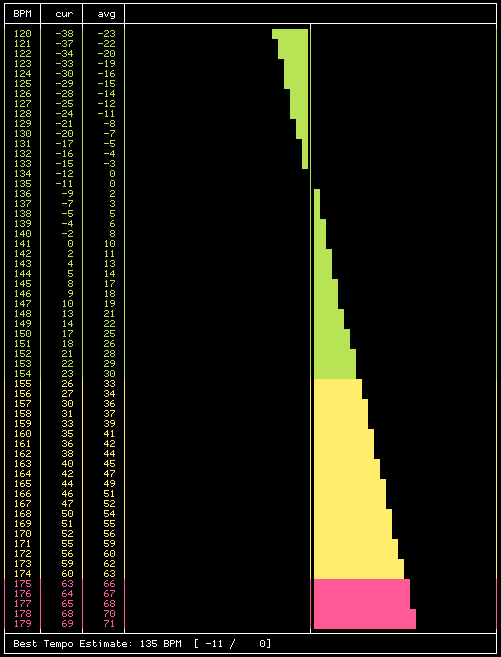
\includegraphics[scale=0.4]{fig/swss.png}
        \caption{software interface screenshot showing a 134~BPM song}
        \label{fig:swss}
    \end{figure}


\section{Evaluation}
    Throughout the project, this project was built very close to the hardware.
    Hardware testing was done just as much, if not more than simulation testing
    throughout the process.  Device timing and area constraints were constantly
    in mind throughout the entire development process.

    After an initial period of testing with only a few metronomes, the design
    was built with over 60 with little issue in regards to timing or area
    constraints.  The metronomes do not perform any complex mathematics at all,
    so it is very easy to fit a lot of them onto even a very weak FPGA.
    Figure~\ref{fig:xst} shows the device utilization.


    \begin{figure}
        \centering
\begin{monospace}
Device utilization summary:
---------------------------

Selected Device : 3s700anfgg484-4 

 Number of Slices:                  2420  out of   5888    41%  
 Number of Slice Flip Flops:        2234  out of  11776    18%  
 Number of 4 input LUTs:            4069  out of  11776    34%  
    Number used as logic:           3893
    Number used as Shift registers:  112
    Number used as RAMs:              64
 Number of IOs:                       36
 Number of bonded IOBs:               26  out of    372     6%  
 Number of MULT18X18SIOs:              3  out of     20    15%  
 Number of GCLKs:                      2  out of     24     8%  
 Number of DCMs:                       1  out of      8    12%  
\end{monospace}
        \caption{device utilization}
        \label{fig:xst}
    \end{figure}

Examining the timing analysis report, the critical path is through the beat
classifier, with the majority of the time is from the energy calculation path.
Figure~\ref{fig:twr} shows the critical path from the timing analysis.

    \begin{sidewaysfigure}
        \centering
\begin{monospace}
Paths for end point beat_tracker_inst/bc_bc_outfifo/empty_reg (SLICE_X51Y29.G4), 8012777023 paths
--------------------------------------------------------------------------------
Slack (setup path):     0.672ns (requirement - (data path - clock path skew + uncertainty))
  Source:               beat_tracker_inst/bc_bc_avg_energy_0 (FF)
  Destination:          beat_tracker_inst/bc_bc_outfifo/empty_reg (FF)
  Requirement:          40.000ns
  Data Path Delay:      39.188ns (Levels of Logic = 68)
  Clock Path Skew:      -0.140ns (0.414 - 0.554)
  Source Clock:         clk25 rising at 0.000ns
  Destination Clock:    clk25 rising at 40.000ns
  Clock Uncertainty:    0.000ns

  Maximum Data Path: beat_tracker_inst/bc_bc_avg_energy_0 to beat_tracker_inst/bc_bc_outfifo/empty_reg
    Location             Delay type         Delay(ns)  Physical Resource
                                                       Logical Resource(s)
    -------------------------------------------------  -------------------
    SLICE_X53Y14.XQ      Tcko                  0.591   beat_tracker_inst/bc_bc_avg_energy<0>
                                                       beat_tracker_inst/bc_bc_avg_energy_0
    SLICE_X52Y13.F2      net (fanout=3)        0.483   beat_tracker_inst/bc_bc_avg_energy<0>
            
                                     . . .

                                                       beat_tracker_inst/Mcompar_NOT_SEXT_bc_bc
                                                        _energy_buf_63_0_11_CONCAT_0_12__ETC___d154_cy<28>
    SLICE_X51Y29.G4      net (fanout=1)        0.652   beat_tracker_inst/Mcompar_NOT_SEXT_bc_bc
                                                        _energy_buf_63_0_11_CONCAT_0_12__ETC___d154_cy<28>
    SLICE_X51Y29.CLK     Tgck                  0.727   beat_tracker_inst/bc_bc_outfifo/empty_reg
                                                       beat_tracker_inst/bc_bc_outfifo/empty_reg_rstpot
                                                       beat_tracker_inst/bc_bc_outfifo/empty_reg
    -------------------------------------------------  ---------------------------
    Total                                     39.188ns (26.200ns logic, 12.988ns route)
                                                       (66.9% logic, 33.1% route)
\end{monospace}
        \caption{timing analysis}
        \label{fig:twr}
    \end{sidewaysfigure}


    A fair amount of code was involved in this project, as shown in
    Figure~\ref{fig:linecount}.  The design used some existing blocks that I
    had built for this FPGA, as well as a UART block originally built by
    Digilent.  The majority of the project goals were met, but the convergence
    time is still not what it needs to be.  The predicted tempo still has
    periods where it fluctuates wildly.  Better handling of situations where
    the beat classifier is not sure what's going on will improve this problem
    drastically, but I unfortunately did not have enough time to complete that.
    I hope to spend more time improving this handling.

    \begin{figure}
        \centering
\begin{monospace}
└──> ./sw/count-lines.sh 
Calculating amount of brainpower spent on bt...

Language   Lines
---------  -----
 Bluespec:   836
     VHDL:  1390
Testbench:    85
    LaTeX:  1455
    Shell:    29
   Python:  1030

    Total:  4825
\end{monospace}
        \caption{summary of code written for \projname}
        \label{fig:linecount}
    \end{figure}

\section{Design Exploration --- Thoughts for the Future}
    \subsection{Estimating Best Tempo}
        Right now, the software interface determines the best tempo estimate
        from the phase errors of the metronomes.  It might be useful to fold
        this into the FPGA itself.  Furthermore, one could use additional
        information that the current design essentially throws out to improve
        tempo estimation.  By paying attention to how likely we're in a part of
        the stream that has a strong beat, we can ignore spurious data more
        easily and get a better estimate of what the true tempo is.

    \subsection{Variance-Sensitive Beat Classifier}
        
        If we store about 1 second worth of energies, we can perform the following
        linear regression to determine a good fit for the ratio of the current
        instantaneous energy to the last second of average energy in order to
        detect a beat.  Thus, we're looking for:

        \begin{align}
            \frac{e}{\mu_E} \geq 1.5142857 - 0.0025714 \sigma^2_E
        \end{align}

        where $\mu_E$ is the average energy, $e$ is the current instantaneous
        energy, and $\sigma^2$ is the variance of the last second's worth of
        energies.  More specifically:

        \begin{align}
            \mu_E &= \frac{1}{n} \sum_{i=0}^{n-1} e_i \\
            \sigma^2_E &= \mu_{E^2} - (\mu_E)^2
        \end{align}

        We can rearrange these equations to be more suitable for implementation in
        a digital system:

        \begin{align}
            e \geq & 1.5142857 \mu_E  - 0.0025714 \sigma^2_E \mu_E \\
            \geq & 1.5142857 \mu_E
                    - 0.0025714 (\mu_{E^2} - (\mu_E)^2) \mu_E \\
            \geq & 1.5142857 \mu_E
                    - 0.0025714 \mu_E \mu_{E^2} 
                    + 0.0025714 (\mu_E)^3 \\
            \geq & 1.5142857 \frac{1}{n} \sum_{i=0}^{n-1} e_i \\
                & - 0.0025714 \left[
                                    \left(\frac{1}{n} \sum_{i=0}^{n-1} (e_i)^2\right) +
                                    \left(
                                        \left(\frac{1}{n} \sum_{i=0}^{n-1} e_i\right) \cdot
                                        \left(\frac{1}{n} \sum_{i=0}^{n-1} e_i\right)
                                    \right)
                                \right] \cdot
                                \left(\frac{1}{n} \sum_{i=0}^{n-1} e_i\right)
        \end{align}


        So, if we keep a shift register of the last $n$ energies, as well as the
        last $n$ energies squared, as well as a running sum of those two, then we
        can simply subtract the oldest value and add the newest value with each new
        input energy.  This allows us to quickly compute variance with just one
        extra cycle.  From there, we can use Bluespec's \ttt{FixedPoint} library to
        compute the value of $e$ in two more cycles (I'm limiting one
        multiplication per cycle due to resource constraints on the FPGA.  We then
        can compare $e$ to the current instantaneous energy to see if a beat event
        occurred or not.

        The current design does this in 4 linearly-pipelined stages, though
        eventually failed to meet the resource constraints of the FPGA.  I'm
        exploring alternate designs.

    \subsection{Frequency-Aware Beat Classifier}

        A far better beat classifier uses frequency data to determine beat
        likelihood.  This helps offset problems that occur in music where two
        instruments alternate.

    \subsection{Final Thoughts}

        I intend to continue working on this project for as long as I can get
        access to a Bluespec license, which unfortunately won't be for long
        given that I'm graduating this year.

\end{document}
